
\section{Deep Feature Learning}
\label{ex:3}


\subsection{Stacked Autoencoders}
\label{ex:3.1}

\begin{task}{3.1.1}
  % Conduct image classification on MNIST using an stacked autoencoder. Are you able to obtain a
  % better result by changing the size of the network architecture? What are the results before and
  % after fine-tuning? What is the benefit of pretraining the network layer by layer?
\end{task}

I am using two autoencoders stacked on top of each other with hidden dimensions $256$ and $64$
respectively. Changing the size of the network architecture did not yield significant improvements.
Changing the number of epochs however did. I got the best results with $20$ epochs for pre-training
each layer, $30$ epochs to train the classification layer and $50$ epochs to fine-tune the whole
network. The loss for every training step is shown in Figure~\ref{fig:ex3_1_loss}. Fine-tuning
significantly improved the performance. The accuracy on the test set was $0.955$. Pretraining the
network layer by layer helps to find a good initialization for the weights. This seems to work
well in this case. However, the network was not able to learn by training the classification layer.

\begin{figure}[ht!]
  \centering
  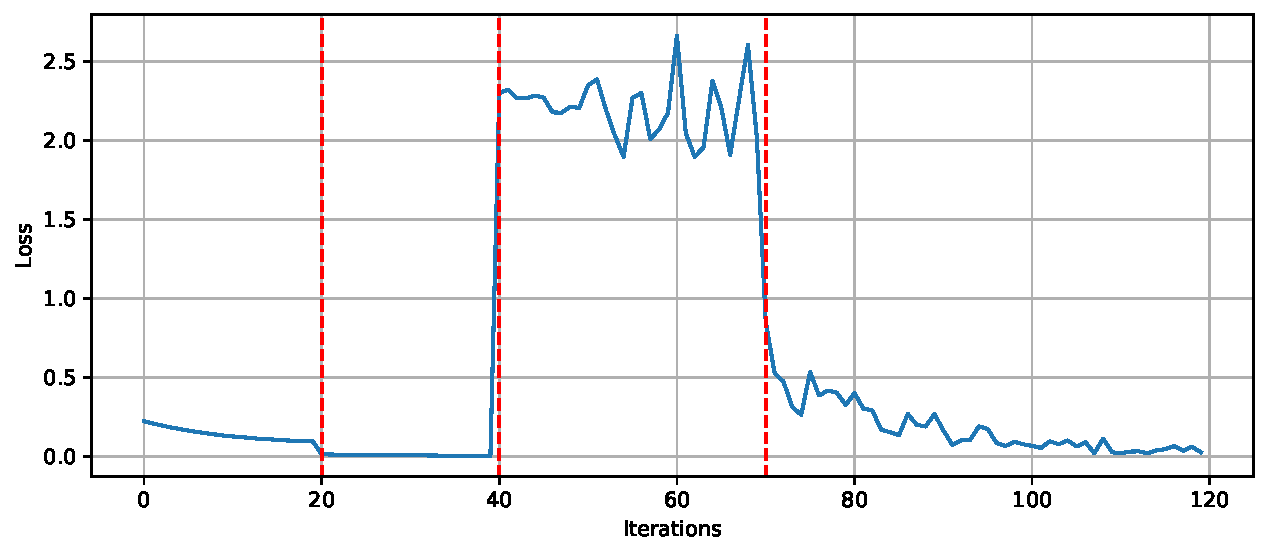
\includegraphics[width=0.9\textwidth]{ex3_1_loss.pdf}
  \caption{Loss for the stacked autoencoder. (1) Pre-training the first layer, (2) pre-training the
    second layer, (3) training the classification layer, (4) fine-tuning the whole network.}
  \label{fig:ex3_1_loss}
\end{figure}

% WITH epochs = (10, 10, 20)
% hidden_dim1 = 256
% hidden_dim2 = 64
% -> Accuracy on the test set: 0.918, last loss: 0.1718
% hidden_dim1 = 128
% hidden_dim2 = 32
% -> Accuracy on the test set: 0.924, last loss: 0.1339
% hidden_dim1 = 128
% hidden_dim2 = 64
% -> Accuracy on the test set: 0.916, last loss: 0.2189
% hidden_dim1 = 64
% hidden_dim2 = 16
% -> Accuracy on the test set: 0.923, last loss: 0.1196
% hidden_dim1 = 64
% hidden_dim2 = 32
% -> Accuracy on the test set: 0.937, last loss: 0.1227
% hidden_dim1 = 32
% hidden_dim2 = 16
% -> Accuracy on the test set: 0.923, last loss: 0.0933
% hidden_dim1 = 32
% hidden_dim2 = 32
% -> Accuracy on the test set: 0.925, last loss: 0.1617
% hidden_dim1 = 128
% hidden_dim2 = 16
% -> Accuracy on the test set: 0.928, last loss: 0.2104
% hidden_dim1 = 64
% hidden_dim2 = 48
% -> Accuracy on the test set: 0.926, last loss: 0.1306
% WITH epochs = (20, 30, 50)
% hidden_dim1 = 512
% hidden_dim2 = 256
% -> Accuracy on the test set: 0.947
% hidden_dim1 = 256
% hidden_dim2 = 64
% -> Accuracy on the test set: 0.955

\subsection{Convolutional Neural Networks}
\label{ex:3.2}

\begin{task}{3.2.1}
  %   Answer the following questions:
  % • Consider the following 2D input matrix.
  %  \mathbf {X} = \begin {bmatrix} 2 & 5 & 4 & 1 \\ 3 & 1 & 2 & 0 \\ 4 & 5 & 7 & 1 \\ 1 & 2 & 3 & 4 \end {bmatrix},
  % Calculate the output of a convolution with the following 2x2 kernel with no padding and a stride
  % of 2.
  %  \mathbf {K} = \begin {bmatrix} 1 & 0 \\ 0 & 1 \\ \end {bmatrix}.
  % • How do you in general determine the dimensionality of the output of a convolutional layer?
  % • What benefits do CNNs have over regular fully connected networks?
\end{task}

\begin{enumerate}[(a)]
  \item The output of the convolution is calculated as follows:
        \begin{align}
          \mathbf{X} * \mathbf{K} & = \begin{bmatrix}
                                        2 & 5 & 4 & 1 \\
                                        3 & 1 & 2 & 0 \\
                                        4 & 5 & 7 & 1 \\
                                        1 & 2 & 3 & 4
                                      \end{bmatrix} * \begin{bmatrix}
                                                        1 & 0 \\
                                                        0 & 1
                                                      \end{bmatrix}                \\
                                  & = \begin{bmatrix}
                                        2*1 + 5*0 + 3*0 + 1*1 & 4*1 + 1*0 + 2*0 + 0*1 \\
                                        4*1 + 5*0 + 1*0 + 2*1 & 7*1 + 1*0 + 3*0 + 4*1
                                      \end{bmatrix} \\
                                  & = \begin{bmatrix}
                                        3 & 4  \\
                                        6 & 11
                                      \end{bmatrix}
        \end{align}
  \item Let $X \in \mathbb{R}^{n \times n}$ be the input matrix, $K \in \mathbb{R}^{m \times m}$ the
        kernel, $P \in \mathbb{N}$ the padding, $S \in \mathbb{N}$ the stride and $Y \in
          \mathbb{R}^{k \times k}$ the output matrix. Then the dimensionality of the output is
        determined by
        \begin{equation}
          k = \left\lfloor \frac{n - m + 2P}{S} \right\rfloor + 1
        \end{equation}
  \item The big benefit is that, compared to fully connected networks, CNNs have way fewer
        parameters. This is because the weights are shared across the input. It also allows the
        network to capture how pixels are spatially related to each other. This is especially useful
        for image data.
\end{enumerate}


\begin{task}{3.2.2}
  % The file cnn.ipynb runs a small CNN on the handwritten digits dataset (MNIST). Use this script
  % to investigate some CNN architectures. Try out different amounts of layers, combinations of
  % different kinds of layers, number of filters and kernel sizes. Note that emphasis is not on
  % experimenting with batch size or epochs, but on parameters specific to CNNs. Pay close attention
  % when adjusting the parameters for a convolutional layer as the dimensions of the input and
  % output between layers must align. Discuss your results. Please remember that some architectures
  % will take a long time to train.
\end{task}

The final architecture has the following layers:\\[0.5em]
\begin{minipage}[t]{0.48\linewidth}
  \begin{enumerate}
    \item \textbf{Convolutional layer}
          \begin{itemize}
            \item Number of filters: $16$
            \item Kernel size: $(4, 4)$
            \item Stride: $(2, 2)$
            \item Padding: $(2, 2)$
            \item Batch normalization
            \item ReLU activation
            \item Dropout with probability $0.2$
          \end{itemize}
    \item \textbf{Convolutional layer}
          \begin{itemize}
            \item Number of filters: $32$
            \item Kernel size: $(4, 4)$
            \item Stride: $(2, 2)$
            \item Padding: $(1, 1)$
            \item Batch normalization
            \item ReLU activation
            \item Dropout with probability $0.4$
          \end{itemize}
  \end{enumerate}
\end{minipage}
\begin{minipage}[t]{0.48\linewidth}
  \begin{enumerate}
    \setcounter{enumi}{2}
    \item \textbf{Convolutional layer}
          \begin{itemize}
            \item Number of filters: $32$
            \item Kernel size: $(3, 3)$
            \item Stride: $(1, 1)$
            \item Padding: $(1, 1)$
            \item Batch normalization
            \item ReLU activation
            \item Dropout with probability $0.4$
          \end{itemize}
    \item \textbf{Convolutional layer}
          \begin{itemize}
            \item Number of filters: $64$
            \item Kernel size: $(2, 2)$
            \item Stride: $(1, 1)$
            \item Batch normalization
            \item ReLU activation
          \end{itemize}
    \item \textbf{Fully connected layer} with $2304$ inputs and $100$ outputs
    \item \textbf{Fully connected layer} with $100$ inputs and $10$ outputs
  \end{enumerate}
\end{minipage}
\vspace*{0.3cm}

This architecture is the result of various experiments. I tested different output channels, kernel
sizes, strides, padding, activation functions, dropout rates, batch normalization and pooling. The
most important factors for the performance were the number of filters, bigger kernel sizes and
dropout.\\
Adding more layers did not improve the performance. Too many parameters would lead to overfitting.
This was also the case with bigger kernel sizes, but dropout helped to prevent this. Without
dropout, the accuracy increased fast but stagnated quickly. Pooling increased the variance in the
accuracy a lot. I tested the activation functions ReLU, Sigmoid and Tanh. ReLU performed the best.
Batch normalization only improved the performance a little. The results of different kernel sizes,
strides and padding were hard to interpret. The results were inconsistent, but had a small tendency
that suggested that using a bigger kernel size in the first layers and smaller kernel sizes in the
following layers worked best. To prevent too many parameters, I used strides of $2$ in the first
layers. Test accuracy was used as the main metric to evaluate the performance. The architecture
above achieved an accuracy of $99.0\%$.


\vspace*{1em}
\subsection{Self-Attention and Transformers}
\label{ex:3.3}


\begin{task}{3.3.1: Self-Attention Mechanism}
  % Please run both the NumPy and PyTorch implementations of the self-attention mechanism. Can you
  % explain briefly how the dimensions between the queries, keys and values, attention scores and
  % attention outputs are related? What do the query, key and value vectors represent? Note that the
  % attention mechanism will also be discussed in lecture 11.
\end{task}

The self-attention mechanism was introduced by Vaswani et al. in 2017, where they define the
attention function for a set of queries.\\
Let $\mathbf{X} \in \mathbb{R}^{N \times d_e}$ be the input, where $N$ is the number of tokens and
$d_e$ is the dimension of the word embeddings. Let $\mathbf{W}_q, \mathbf{W}_k \in \mathbb{R}^{d_e
    \times d_k}$ and $\mathbf{W}_v \in \mathbb{R}^{d_e \times d_v}$ be the weight matrices for the
queries, keys and values respectively. The dimensions of the queries, keys and values are related as
follows:
\begin{equation}
  \mathbf{Q} = \mathbf{X} \mathbf{W}_q \in \mathbb{R}^{N \times d_k}, \quad
  \mathbf{K} = \mathbf{X} \mathbf{W}_k \in \mathbb{R}^{N \times d_k}, \quad
  \mathbf{V} = \mathbf{X} \mathbf{W}_v \in \mathbb{R}^{N \times d_v}
\end{equation}
\begin{equation}
  \mathbf{Q} \mathbf{K}^T \in \mathbb{R}^{N \times N}, \quad
  \text{softmax}\left( \frac{\mathbf{Q} \mathbf{K}^T}{\sqrt{d_k}} \right) \in \mathbb{R}^{N \times N}
\end{equation}
The attention output is then calculated as follows:
\begin{equation}
  \text{Attention}(\mathbf{Q}, \mathbf{K}, \mathbf{V}) = \text{softmax}\left( \frac{\mathbf{Q}
    \mathbf{K}^T}{\sqrt{d_k}} \right) \mathbf{V} \in \mathbb{R}^{N \times d_v}
\end{equation}

The query, key and value vectors represent the input in different spaces. The query vector encodes
what the model is looking for, like a question that expresses your intrest. The key vector encodes
the characteristics of all available information. The value vector represents the actual
information you will use. This way the model can learn to focus on the relevant parts of the input
and ignore the rest.



\begin{task}{3.3.2: Transformers}
  % Please train the Transformer on the MNIST dataset. You can try to change the architecture by
  % tuning dim, depth, heads, mlp dim for better results. You can try to increase or decrease the
  % network size and see whether it will influence the prediction results much. Note that ViT can
  % easily overfit on small datasets due to its large capacity. Discuss your results under different
  % architecture sizes.
\end{task}

\begin{table}[htbp]
  \begin{center}
    \begin{tabular}{|c|c|c|c|c|c|}
      \hline
      \textbf{Rank} & \textbf{\texttt{dim}} & \textbf{\texttt{depth}} & \textbf{\texttt{mlp\_dim}} & \textbf{\texttt{accuracy}} & \textbf{\texttt{Exec Time}} \\
      \hline
      1             & 128                   & 8                       & 128                        & 0.9871                     & 351.1s                      \\
      \hline
      2             & 128                   & 6                       & 256                        & 0.9863                     & 309.6s                      \\
      \hline
      3             & 128                   & 4                       & 512                        & 0.9860                     & 455.0s                      \\
      \hline
      4             & 256                   & 4                       & 512                        & 0.9859                     & 730.3s                      \\
      \hline
      5             & 128                   & 8                       & 64                         & 0.9857                     & 351.4s                      \\
      \hline
      6             & 64                    & 8                       & 128                        & 0.9856                     & 356.4s                      \\
      \hline
      7             & 64                    & 4                       & 128                        & 0.9851                     & 264.4s                      \\
      \hline
      8             & 64                    & 8                       & 256                        & 0.9849                     & 355.6s                      \\
      \hline
      9             & 64                    & 6                       & 128                        & 0.9847                     & 310.6s                      \\
      \hline
      10            & 32                    & 8                       & 128                        & 0.9845                     & 350.2s                      \\
      \hline
      11            & 128                   & 6                       & 128                        & 0.9842                     & 500.1s                      \\
      \hline
      12            & 128                   & 8                       & 256                        & 0.9841                     & 352.6s                      \\
      \hline
      13            & 256                   & 8                       & 64                         & 0.9839                     & 999.3s                      \\
      \hline
      14            & 128                   & 10                      & 64                         & 0.9838                     & 710.6s                      \\
      \hline
      15            & 128                   & 6                       & 64                         & 0.9837                     & 311.1s                      \\
      \hline
      16            & 128                   & 4                       & 256                        & 0.9837                     & 270.3s                      \\
      \hline
      17            & 32                    & 10                      & 256                        & 0.9835                     & 605.7s                      \\
      \hline
      18            & 64                    & 8                       & 64                         & 0.9835                     & 356.8s                      \\
      \hline
      19            & 64                    & 4                       & 64                         & 0.9834                     & 281.3s                      \\
      \hline
      20            & 128                   & 10                      & 128                        & 0.9833                     & 758.1s                      \\
      \hline
      21            & 32                    & 8                       & 256                        & 0.9833                     & 353.7s                      \\
      \hline
      22            & 128                   & 4                       & 128                        & 0.9833                     & 269.3s                      \\
      \hline
      23            & 64                    & 6                       & 256                        & 0.9831                     & 461.7s                      \\
      \hline
      24            & 256                   & 10                      & 128                        & 0.9831                     & 1302.0s                     \\
      \hline
      25            & 128                   & 4                       & 64                         & 0.9829                     & 268.8s                      \\
      \hline
      26            & 32                    & 8                       & 64                         & 0.9829                     & 351.6s                      \\
      \hline
      27            & 256                   & 8                       & 128                        & 0.9827                     & 1067.3s                     \\
      \hline
      28            & 64                    & 6                       & 64                         & 0.9827                     & 309.7s                      \\
      \hline
      29            & 32                    & 8                       & 512                        & 0.9820                     & 529.6s                      \\
      \hline
      30            & 32                    & 6                       & 128                        & 0.9819                     & 311.4s                      \\
      \hline
      31            & 32                    & 6                       & 64                         & 0.9816                     & 313.3s                      \\
      \hline
      32            & 64                    & 4                       & 256                        & 0.9816                     & 267.8s                      \\
      \hline
      33            & 256                   & 10                      & 256                        & 0.9815                     & 1432.3s                     \\
      \hline
      34            & 32                    & 6                       & 256                        & 0.9809                     & 403.2s                      \\
      \hline
      35            & 32                    & 4                       & 512                        & 0.9808                     & 301.9s                      \\
      \hline
      36            & 32                    & 4                       & 256                        & 0.9808                     & 266.2s                      \\
      \hline
      37            & 64                    & 4                       & 512                        & 0.9807                     & 358.5s                      \\
      \hline
      38            & 32                    & 4                       & 128                        & 0.9798                     & 266.7s                      \\
      \hline
      39            & 32                    & 4                       & 64                         & 0.9788                     & 268.2s                      \\
      \hline
      40            & 32                    & 6                       & 512                        & 0.9778                     & 418.6s                      \\
      \hline
    \end{tabular}
  \end{center}
  \caption{Accuracy of different Transformer models on MNIST dataset}
  \label{tab:transformer_accuracy}
\end{table}

\begin{figure}
  \centering
  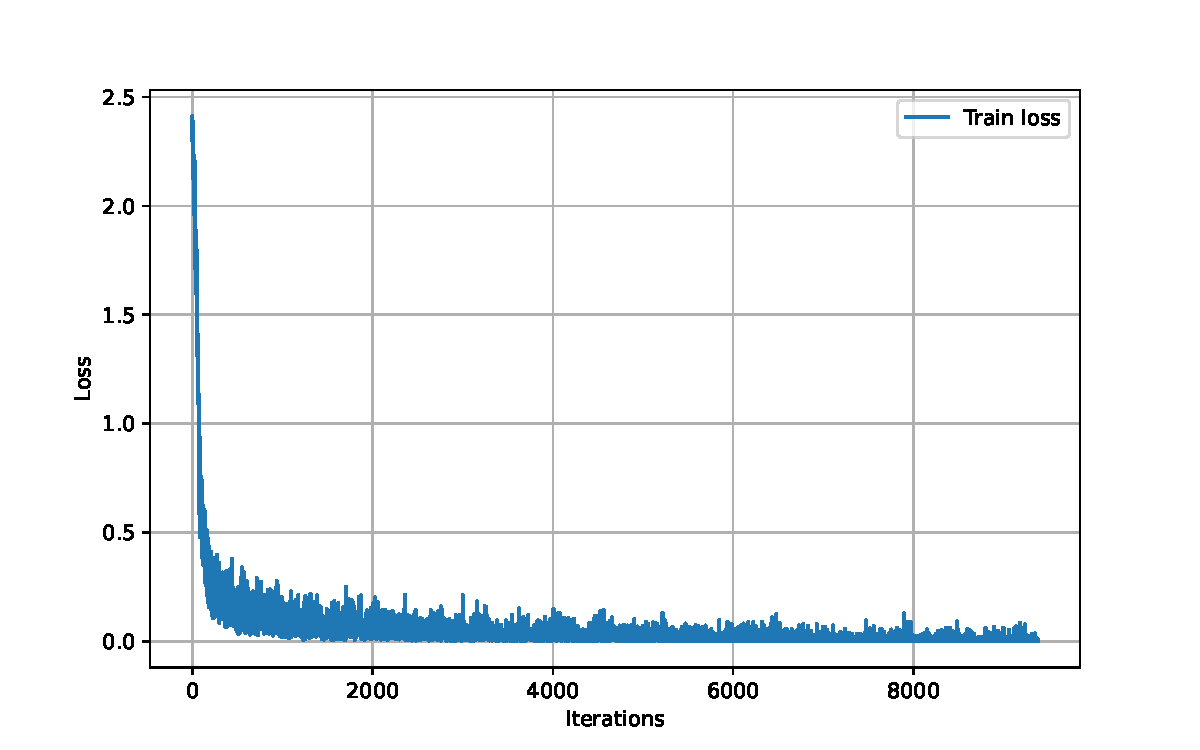
\includegraphics[width=0.6\textwidth]{ex3_3_train_loss.pdf}
  \caption{Training loss of the best Transformer model.}
  \label{fig:ex3_3_train_loss}
\end{figure}

To find the best architecture, I did a grid search over the parameters \texttt{dim}, \texttt{depth}
and \texttt{mlp\_dim}, because these are the most important parameters. I kept the number of heads
fixed at $8$, the batch size at $128$ and the number of epochs at $20$. The results are shown in
Table~\ref{tab:transformer_accuracy}. Comparing the results of the different architectures, one can
see that the accuracy is very similar for most of them. The training time however increases with the
number of dimensions. The parameter \texttt{dim} has the biggest impact on the accuracy. A bigger
dimensionality leads to better results. The depth and the MLP dimension have a smaller impact.\\
The best model had a dimension of $128$, a depth of $8$ and an MLP dimension of $128$. The accuracy
on the test set was $0.9871$. The training loss shows a lot of variance, but the model was able to
learn. The training loss is shown in Figure~\ref{fig:ex3_3_train_loss}.
